\documentclass{article}
\usepackage[utf8]{inputenc}
\usepackage{float}
\usepackage{lipsum}
\usepackage{mwe}
\title{EditDistance e indici n-gram}
\author{Luca Maltempo}
\date{October 2021}

\begin{document}

\maketitle

\section{Introduzione}
L'algoritmo Edit Distance permette di calcolare la distanza tra due parole di un dizionario, questo algoritmo, implementato attraverso diverse tecniche, viene usato da molti programmi di scrittura, affinché possa riconoscere eventuali errori di battitura e correggerli consigliando le parole del dizionario che sono più vicine a quella che è stata digitata. In generale vogliamo che l'operazione di calcolo della distanza tra una parola e le restanti del dizionario sia molto veloce, questo perchè abbiamo bisogno che la correzione della parola errata sia fatta in tempo reale.
\section{Edit Distance}
L'algoritmo riceve due stringhe di caratteri X e Y e calcola la loro distanza di edit che è pari al minimo numero di operazioni elementari necessarie per far in modo che le due stringhe abbiano lo stesso contenuto. Ogni operazione ha un costo che poi determina la distanza effettiva tra le due parole.

Operazioni elementati e costo:
\begin{itemize}
    \item Copia, 0 = Lascia invariato un carattere e ha costo nullo.
    \item Sostituzione, 1 = Sostituisce un carattere della prima stringa col carattere corrispondente della seconda stringa. 
    \item Scambio, 1 = Scambia due caratteri di una stringa se questi risultano in posizioni invertite nella seconda stringa. 
    \item Cancellazione, 1 = Cancella un carattere da una stringa.
    \item Inserimento, 1 = Inserisce un carattere in una stringa.
\end{itemize}
Come per il problema della massima sottosequenza comune (LCS), anche in questo caso è possibile definire una sottostruttura ottima valutando le due stringhe un carattere alla volta. Sia m la lunghezza di X e n la lunghezza di Y, definiamo $X_{i}= < x_{0}, x_{1},...,x_{i} >$ e  $Y_{j}= < y_{0}, y_{1},...,y_{j} >$ sottosequenze di X e Y.
I sottoproblemi da risolvere sono il calcolo della distanza di edit sulle sottosequenze $X_{i}$ e $Y_{j}$ per i, j = 0, 1,..., m, n.
Una soluzione ottima al problema $X_{i}$ $\rightarrow$ $Y_{j}$ deve includere una soluzione ottima al problema $X_{i-1}$ $\rightarrow$ $Y_{j-1}$. Definisco C[i][j] il costo di una soluzione ottima al problema $X_{i}$ $\rightarrow$ $Y_{j}$ nel seguente modo: C[i][j] = C[i-1][j-1] + costo(operazione). Attraverso una formulazione ricorsiva arriviamo alla risoluzione del problema di Edit-Distance in un tempo pari a $\theta(m \cdot n)$ % regular O .

\section{Utlizzare l'Edit Distance}
L'edit distance per la ricerca della parola più vicina ad una query può essere implementata in diversi modi. La tecnica più naive vede l'esecuzione dell'algoritmo su tutte le parole del dizionario. Di solito si tende ad evitare questa tecnica se è necessario che l'algoritmo venga eseguito in tempi rapidi. Per velocizzare l'esecuzione dell'Edit-Distance si fa affidamento agli indici n-gram.
\subsection{N-gram}
L' n-gram di una parola corrisponde all'insieme di tutte le sottosequenze di lunghezza n della parola.
La creazione degli indici n-gram di tutte le parole del dizionario permette un utilizzo più furbo dell'edit-distance. Infatti, invece di eseguire il calcolo della distanza tra la query e tutte le parole del dizionario, l'edit distance è eseguita solo nel caso in cui le due parole abbiano un numero sufficientemente alto di sottosequenze in comune. Date due stringhe, definisco con X e Y i rispettivi insiemi di sottosequenze di lunghezza n, e ricavo il Coefficiente di Jaccard tramite questa formula: J = $\frac{X\cap Y}{X \cup Y}$ . L'edit Distance tra le due parole viene realizzato solo se il coefficiente di Jaccard è superiore ad una soglia di valore arbitrario. Maggiore è questa soglia e minore sarà il numero di edit distance che vengono eseguiti, in questo modo si riesce a diminuire in modo considerevole il tempo di esecuzione dell'algoritmo ma si va anche a diminuire il suo Hit Rate. 
\section{Esperimenti svolti}
Per testare l' efficacia dei diversi algoritmi implementati nel codice è stato utilizzato un dizionario contenente 95 mila parole italiane, tra queste sono presenti anche nomi propri e località. Ovviamente, il tempo di esecuzione dell'Edit Distance varia molto in base alla lunghezza del dizionario utilizzato oltre che alla tecnica scelta per l'implementazione dell'algoritmo. Per reallizare i vari test vengono inserite in una lista 100 parole scelte casualemnte dal dizionario. A partire da questa lista con le parole originarie vengono costruite 5 nuove liste, ognuna contenente le parole originarie modicate in $n$ caratteri, con $n =1,..,5$. Ogni parola viene modificata attraverso operazioni elementari come l'inserimento di un carattere, eliminazione di un carattere, sostituzione di carattere con un altro dell'alfabeto o scambio di un carattere col precedente. Le liste con le parole modificate servono a simulare eventuali errori di battitura. A questo punto non rimane altro che calcolare l'edit distance su ogni parola modificata e vedere se le parole a distanza minore corrispondono a quella originaria, Hit, o meno, Miss.
L'edit distance è stata implementata in 2 diverse modalità, la versione naive prevede l'edit distance tra la parola modificata e l'intero dizionario mentre la seconda versione sfrutta gli indici n-gram, per la precisione 2-gram, 3-gram e 4-gram, e realizza l'edit distance tra la parola modificata e una del dizionario solo se il loro coefficiente di Jaccard è maggiore della soglia indicata. Per l'esperimento sono state scelte tre soglie: 0.2, 0.4 e 0.8 .
L'Hit Rate mostrato nei risultati sperimentali equivale al rapporto tra il numero di parole modificate per le quali l'Edit Distance ha avuto successo e il numero totale di parole considerate nell'esperimento, in questo caso 100.

\section{Risultati sperimentali}

\begin{table}[h]
    \centering
    \begin{tabular}{|p{3cm}||p{3cm}|p{3cm}|}
        \hline
        \multicolumn{3}{|c|}{Edit Distance su dizionario intero} \\
        \hline
        Numero di caratteri modificati &Hit Rate& Tempo \\
        \hline
        $n = $ 1 & 0.99 & 86 \\                                            
        $n = $ 2 & 0.94 & 89  \\                                                 
        $n = $ 3 & 0.82  & 86 \\                                                
        $n = $ 4 & 0.67  & 85 \\                                     
        $n = $ 5 & 0.57  & 91 \\                                                        \hline
    \end{tabular}
    \caption{Hit rate e tempo di esecuzione(s) dell'Edit Distance sul dizionario completo al variare del numero di caratteri modificati $n$.}
    \label{tab:my_label}
\medskip
\medskip
\medskip

\centering
\begin{tabular}{ |p{3cm}||p{3cm}|p{3cm}|p{3cm}|  }
 \hline
 \multicolumn{4}{|c|}{Edit Distance con $n = 1$ caratteri modificati} \\
 \hline
Indici n-Gram&Jaccard Treshold $>=0.2$ &Jaccard Treshold $>=0.4$&Jaccard Treshold $>=0.8$ \\
 \hline
 2-Gram   & $h$ = 0.99, $t$ = 2.60    &$h$ = 0.97, $t$ = 0.48 &   $h$ = 0.28, $t$ = 0.41\\
 3-Gram &  $h$ = 0.98, $t$ = 0.64  & $h$ = 0.91, $t$ = 0.37   &$h$ = 0.13, $t$ = 0.37\\
 4-Gram &$h$ = 0.92, $t$ = 0.40 & $h$ = 0.67, $t$ = 0.32 &  $h$ = 0.08, $t$ = 0.30\\
 \hline
\end{tabular}
\caption{Hit rate $h$ e i tempi di esecuzione $t$ dell' Edit Distance attraverso indici n-Gram al variare della soglia di Jaccard, numero di caratteri modificati $n = 1$.}
\end{table}

\makeatletter
\setlength{\@fptop}{0pt}
\makeatother

\begin{table}[t]
\centering
\begin{tabular}{ |p{3cm}||p{3cm}|p{3cm}|p{3cm}|  }
 \hline
 \multicolumn{4}{|c|}{Edit Distance con $n = 2$ caratteri modificati} \\
 \hline
Indici n-Gram&Jaccard Treshold $>=0.2$ &Jaccard Treshold $>=0.4$&Jaccard Treshold $>=0.8$ \\
 \hline
 2-Gram   & $h$ = 0.93, $t$ = 1.82    &$h$ = 0.82, $t$ = 0.45 &   $h$ = 0.04, $t$ = 0.43\\
 3-Gram &  $h$ = 0.83, $t$ = 0.52  & $h$ = 0.33, $t$ = 0.38   &$h$ = 0.04, $t$ = 0.37\\
 4-Gram &$h$ = 0.54, $t$ = 0.36 & $h$ = 0.18, $t$ = 0.18 &  $h$ = 0.04, $t$ = 0.32\\
 \hline
\end{tabular}
\caption{Hit rate $h$ e i tempi di esecuzione $t$ dell' Edit Distance attraverso indici n-Gram al variare della soglia di Jaccard, numero di caratteri modificati $n = 2$.}
\medskip
\medskip
\centering
\begin{tabular}{ |p{3cm}||p{3cm}|p{3cm}|p{3cm}|  }
 \hline
 \multicolumn{4}{|c|}{Edit Distance con $n = 3$ caratteri modificati} \\
 \hline
Indici n-Gram&Jaccard Treshold $>=0.2$ &Jaccard Treshold $>=0.4$&Jaccard Treshold $>=0.8$ \\
 \hline
 2-Gram   & $h$ = 0.78, $t$ = 1.68    &$h$ = 0.54, $t$ = 0.45 &   $h$ = 0.02, $t$ = 0.42\\
 3-Gram &  $h$ = 0.55, $t$ = 0.45  & $h$ = 0.19, $t$ = 0.37   &$h$ = 0.00, $t$ = 0.37\\
 4-Gram &$h$ = 0.34, $t$ = 0.33 & $h$ = 0.08, $t$ = 0.31 &  $h$ = 0.00, $t$ = 0.32\\
 \hline
\end{tabular}
\caption{Hit rate $h$ e i tempi di esecuzione $t$ dell' Edit Distance attraverso indici n-Gram al variare della soglia di Jaccard, numero di caratteri modificati $n = 3$.}
\end{table}


\begin{figure}
    \centering
    \begin{minipage}{0.45\textwidth}
        
        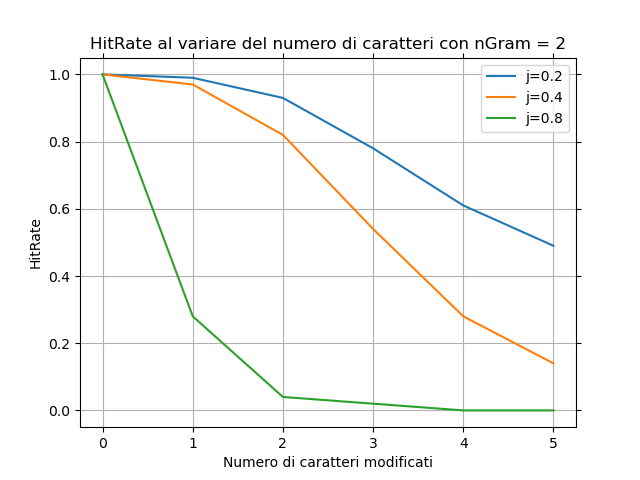
\includegraphics[width=1.35\textwidth]{plotHitRate_nGram2.png} 
        \caption{Grafico Hit Rate con nGram = 2}
    \end{minipage}\hfill
    \begin{minipage}{0.45\textwidth}
       
        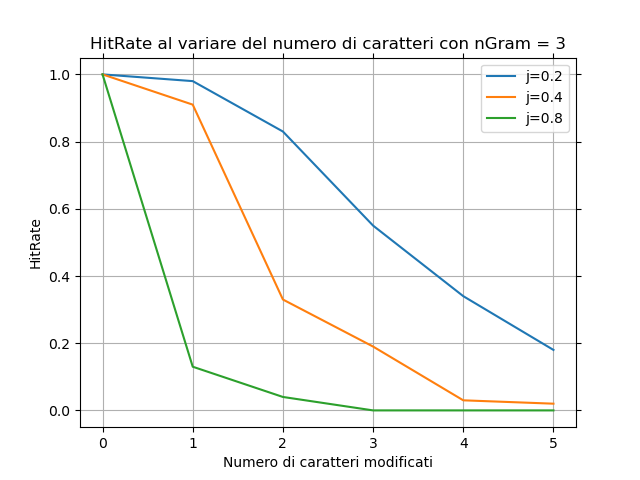
\includegraphics[width=1.35\textwidth]{plotHitRate_nGram3.png} 
        \caption{Grafico Hit Rate con nGram = 3}
    \end{minipage}
\end{figure}


\clearpage

\section{Conclusioni}
Si osserva che, per applicazioni real time, l'implementazione classica dell'Edit distance non sia utilizzabile. Infatti, nonostante abbia registrato l'Hit Rate più alto, impiega quasi un minuto e mezzo per essere eseguita. \newline
Sfuttare gli indici n-Gram  permette invece di ridurre in maniera considerevole il tempo necessario per l'esecuzione dell'algoritmo. Dai risultati è evidente che le combinazioni migliori per ottenere un Hit Rate elevato e un breve tempo di esecuzione siano due, 3-Gram con soglia di Jaccard $>=0.2$ o indici 2-Gram con soglia di Jaccard $>=0.4$, entrambe hanno un tempo di Edit Distance pari a mezzo secondo e mantengono un Hit Rate elevato.


\end{document}
